\section{MHDP Algorithm}
The Multi-objective Hybrid Differential-evolution and Particle-swarm-optimization algorithm combines DE and PSO into a multi-objective optimization algorithm. 
This algorithm is composed of 5 tasks : Solution Coding, Population Initialization, Evaluation of individuals, Mutation and Crossover.
\subsection{Solution Coding}
Each solution is encoded into a vector of $N$ elements whose $i-$th element indicates the number of vehicles sent to the fire point at location $i$.
\subsection{Generating the initial population}
Each individual is created by generating $N$ random integer values, where the random values are chosen in the range \([L_i, U_i]\) to comply with constraint (\ref{eqn:constraints_a}). 
This procedure is repeated until the individual comply also with constraint (\ref{eqn:constraints_b}).
$PopSize$ individuals are generated.
\subsection{Calculating Fitness Values and Screening Pareto Solutions}
After having generated the initial population we compute the fitness value of each solution and we update the personal best \((P_{best})\) value of each individual and the global best value \((G_{best})\).
Subsequently, we seek for Pareto non-dominated solutions (based on fitness value) and we insert the first front in an archive \(A(g)\) responsible for containing the best solutions found until generation \(g\).
Finally, we screen again the Pareto front in the archive because after the insertion of the new individuals there may be new domination relations between the fresh Pareto Solutions and $A(g-1)$.
\subsection{Mutation and Crossover}
A 3-parent mutation strategy is used:
\begin{equation}
    \label{eqn:differential_operator}
    X_i(g+1) = X_i(g) + F \cdot (X_j(g) - X_k(g))
\end{equation}
where \(F\) is the scaling factor (\(F \in (0, 2)\)), \(X_i(g)\) is the $i-th$ individual in the current population, $i, j, k = 1, 2, ..., PopSize$ and $i \neq j \neq k$.\\
MHDP integrates (\ref{eqn:differential_operator}) into PSO:
\begin{equation}
    \begin{aligned}
    \label{eqn:pso}
    X_i(g+1) = X_i(g) + \Phi[r_1(G_{best} - X_i(g)) \\
    + r_2(P_{best} - X_i(g)) + F(X_j(g) - X_k(g))]
    \end{aligned}
\end{equation}
where $\Phi$ is the $round$ function and $r_1, r_2$ are two random numbers
from a uniform distribution over $[0, 1]$. Here each individual takes a small
step towards $G_{best}$ and a small step towards $P_{best}$. The mutation contribution
is given by  $F(X_j(g) - X_k(g))$ where $X_j(g)$ and $X_k(g)$ are randomly selected.\\
The crossover operation is applied to each individual $X_i$ by selecting another random 
individual $X_k$ in the population and performing the operation $X_{ij} = X_{kj}$ with probability $P_c$ for each $j = 1, 2, ..., N$.\\
After mutation and crossover we adjust the new individuals to meet constraints (\ref{eqn:constraints_a}) and (\ref{eqn:constraints_b}).
\subsection{Updating the archive set}
After mutation and crossover we evaluate again the solutions, we update $P_{best}$ for each individual, $G_{best}$ and the archive $A(g)$.\\
The loop of mutation - crossover - evaluation is repeated until a termination condition is met.
\begin{figure}
    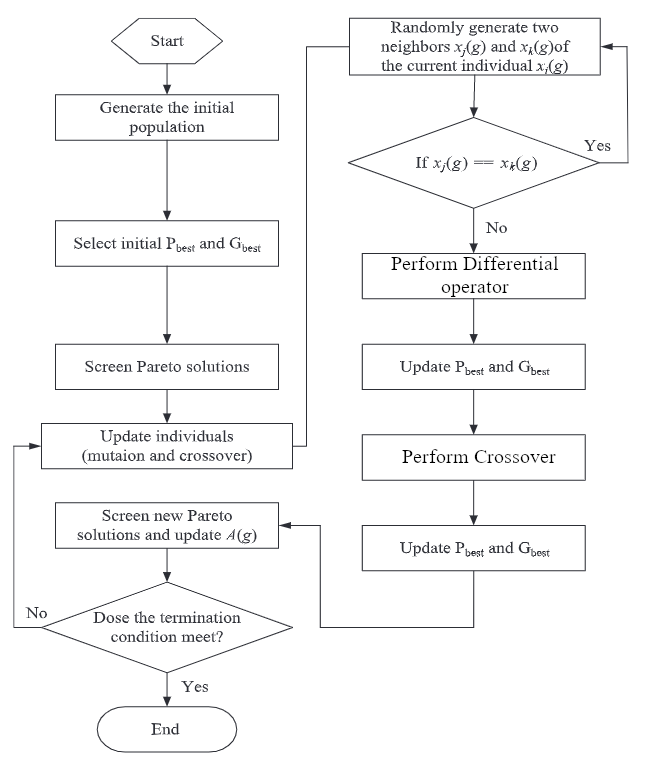
\includegraphics[width=\linewidth]{Images/mhdp_algo.png}
    \caption{MHDP algorithm}
    \label{fig:mhdp}
\end{figure}
